\documentclass[12pt,fleqn]{exam}
\usepackage{pifont}
\usepackage{dingbat}
\usepackage{amsmath,amssymb}
\usepackage{epsfig}
\usepackage[colorlinks=true,linkcolor=black,anchorcolor=black,citecolor=black,filecolor=black,menucolor=black,runcolor=black,urlcolor=black]{hyperref}
\usepackage[letterpaper, margin=0.75in]{geometry}
\addpoints
\boxedpoints
\pointsinmargin
\pointname{pts}

\usepackage{pdfpages}
\usepackage[final]{microtype}
\usepackage[american]{babel}
\usepackage[T1]{fontenc}
\usepackage{fourier}
\usepackage{isomath}
\usepackage{upgreek,amsmath}
\usepackage{amssymb}

\usepackage{graphicx}
\usepackage{color}
\usepackage{tcolorbox}
\newcommand{\dotprod}{\, {\scriptzcriptztyle
    \stackrel{\bullet}{{}}}\,}

\newcommand{\reals}{\mathbf{R}}
\newcommand{\lub}{\mathrm{lub}} 
\newcommand{\glb}{\mathrm{glb}} 
\newcommand{\complex}{\mathbf{C}}
\newcommand{\dom}{\mbox{dom}}
\newcommand{\range}{\mbox{range}}
\newcommand{\cover}{{\mathcal C}}
\newcommand{\integers}{\mathbf{Z}}
\newcommand{\vi}{\, \mathbf{i}}
\newcommand{\vj}{\, \mathbf{j}}
\newcommand{\vk}{\, \mathbf{k}}
\newcommand{\bi}{\, \mathbf{i}}
\newcommand{\bj}{\, \mathbf{j}}
\newcommand{\bk}{\, \mathbf{k}}
\newcommand{\dist}{\, \mathrm{dist}}
\DeclareMathOperator{\Arg}{\mathrm{Arg}}
\DeclareMathOperator{\Ln}{\mathrm{Ln}}
\newcommand{\imag}{\, \mathrm{i}}

\usepackage{xcolor}
\shadedsolutions
\definecolor{SolutionColor}{rgb}{0.95,0.95,0.95}

\usepackage{graphicx}
\newcommand\AM{{\sc am}}
\newcommand\PM{{\sc pm}}
     
%\usepackage{twemojis}
\newcommand{\quiz}{III}
\newcommand{\term}{Spring}
\newcommand{\due}{9:55 \AM}
\newcommand{\class}{MATH 102}
\begin{document}
\large
\vspace{0.1in}
\noindent\makebox[3.0truein][l]{\textbf{\class, \term \/ \the\year}}
\textbf{Name:} \hrulefill \\
\noindent \makebox[3.0truein][l]{\textbf{Review for Exam  \quiz}}
\textbf{Row and Seat}:\hrulefill\\
\vspace{0.1in}


\noindent  Exam \quiz\/  has questions 1 through  \numquestions \/ with a total of  \numpoints\/  points.   

 \noindent \begin{tcolorbox}
    \begin{minipage}{6.5in}
    \begin{enumerate}
    
    \normalsize 
    \item \textbf{Show all of your work.} Do not expect to earn full credit for a correct answer without the needed work.
    
    \item Divine intervention is \emph{not} a substitute for showing your work.
    
    \item If your answer is wrong, but your work shows me that you know the major steps in solving a problem, you will likely earn
    some partial credit.
    
    \item Your work should convince me that not only could you correctly solve the given 
    problem, but you could also solve any related problem.
    
    \item If a question asks for a sentence, write your answer as an English sentence. 
    
    \item No talking, no sharing calculators, and no scratch paper.
    \item  Turn your phone off and put it out of sight.
    \item  Clear your desk of everything, except a pencil, eraser, and a calculator.
    \item If you never make a mistake, you may use ink; otherwise use a pencil.
    \item Do not unstaple the pages of your exam.
    \item We'll all start at the same time--it's the polite thing to do.
    \item Write your answers in the space provided. 
    \item If you do not want something graded, erase it or clearly cross it out. 
    \item You may stare at your feet, your paper, or the ceiling, but nowhere else. 
    \item If you wear a  baseball cap, wear it backwards so I can see your eyes.
    \item Work each problem correctly.
    \item When you are finished, collect your things, place your exam paper in the folder on the front desk,
    and quietly leave the room.
    \item After you turn in your paper, I will not answer questions about the test until after it is graded.
    
    \item Not knowing the rules is not a valid excuse for not following them.
   
    \item Read all directions and problems carefully. 
    \end{enumerate} 
    \end{minipage} 
    
    \end{tcolorbox}
    
    \newpage


\begin{questions} 


\question Find the inverse of the function $f(x) = \frac{2 x + 1}{x-1}, \,\, x \neq 1$.
\begin{solution}[2.5in]

\end{solution}


\question Sketch a pretty good graph of the equation $y = 2 + \left(\frac{1}{2}\right)^x$.
\begin{solution}%[2.5in]

\end{solution}

\vfill
\newpage

    \question Given that $f(x) = 2 x + 3$ and $g(x) = 1-x$, find the 
\emph{numerical value} of each of the following

\begin{parts}
\part [2] $f \circ g (2)$
\begin{solution}[1.25in] We have
  \begin{align*}
      f \circ g(4) &= f(g(4)) & \mbox{(definition of composition)} \\
                   &= f(-3)   & \mbox{(formula for $g$)} \\
                   &= -6 + 3  & \mbox{(formula for $f$)} \\
                   &= -3      & \mbox{(arithematic)}
  \end{align*}

\end{solution}

\part [2] $g \circ f (2)$
\begin{solution}[1.25in]
  \begin{align*}
    g \circ f(4) &= g(f(4)) & \mbox{(definition of composition)} \\
                 &= g(11)   & \mbox{(formula for $f$)} \\
                 &= 1-11     & \mbox{(formula for $g$)} \\
                 &= -10     & \mbox{(arithematic)}
\end{align*}
\end{solution}

\part [2] $g \circ g (1)$
\begin{solution}[1.25in]
  \begin{align*}
    g \circ g(0) &= g(g(0)) & \mbox{(definition of composition)} \\
                 &= g(1)   & \mbox{(formula for $g$)} \\
                 &= 1-1    & \mbox{(formula for $g$)} \\
                 &= 0     & \mbox{(arithematic)}
\end{align*}
\end{solution}


\end{parts}


\question [2] Given that $f(x) = 2 x - 3$ and $g(x) = 1+x$, find 
a formula for $f \circ g$.

\begin{solution} We have
  \begin{align*}
     f \circ g (x) &= f(g(x)) & \mbox{(definition of composition)} \\
                   &= f(1-x)   & \mbox{(formula for $g$)} \\
                   &= 2 (1-x) + 3 & \mbox{(formula for $f$)} \\
                   &= -2x + 5 & \mbox{(simplification)} 
  \end{align*}

\end{solution}
%\hfill
%\newpage 

\question A table of values for functions $f$ and $g$ are

\begin{tabular}[h]{|c|c|} 
  \hline
  $x$  & $f(x)$ \\ \hline \hline
  0    & 3 \\ \hline
  1    & 2 \\ \hline
  2    & 1 \\ \hline
  3    & 0 \\ \hline
\end{tabular} \phantom{xxxxxxx}
\begin{tabular}[h]{|c|c|} 
  \hline
  $x$  & $g(x)$ \\ \hline \hline
  0    & 1 \\ \hline
  1    & 3 \\ \hline
  2    & 0 \\ \hline
  3    & 2 \\ \hline
\end{tabular} 

Find the \emph{numerical values} of 
\begin{parts}
 \part[2] $ f \circ g (1)$
 \begin{solution}[1.25in] These values we just look up!
  \begin{equation*}
    f \circ g (1) = f(g(1)) = f(3) = 0.
  \end{equation*}

 \end{solution}

 \part[2] $ g \circ f (1)$
 \begin{solution}[1.25in]
  \begin{equation*}
    g \circ f (1) = g(f(1)) = g(2) = 2.
  \end{equation*}
 \end{solution}

 \part[2] Using only the values from the table, find the solution
 to the equation \mbox{$g \circ g (x) = 2$.}

 \begin{solution}[1.25in]
   We need to solve the equation $g(g(x)) = 2$. From the table, we see that
   if $g(\mbox{blob}_1) = 2$, then $\mbox{blob}_1 =2$. But $\mbox{blob}_1 =g(x)$,
   so again we need to solve $g(x) = 2$. And that makes $x=2$.

   \textbf{Oops} This problem has too many twos--it's maybe a bit confusing. Let's
   try $g(g(x))=3$. First, we replace $g(x)$ by $\mbox{blob}_1$. So we need to 
   solve $g(\mbox{blob}_1) = 3$. Looking up the input that gives an output of 3,
   we see that $\mbox{blob}_1 = 1$. But $\mbox{blob}_1 = g(x)$, so our new
   problem is $g(x)=1$. Looking up the value that gives an output of 1, we see
   that $x=0$.
 \end{solution}
\end{parts}

\question [2] Given that $E$ is an exponential function and that $E(0)=9$
and $E(1) = 10$, find a formula for $E$.

\begin{solution}[2.5in]  The formula for every exponential function $E$ has the 
    form $E(x) = C a^x$, where $C$ is the initial value and $a$ is the growth rate.
    The fact  $E(0)=9$ tells us that
    \begin{equation*}
        \left[  C a^0 = 9 \right] = \left[  C  = 9 \right]
    \end{equation*}
    So the initial value is $C=9$. And the fact $E(2) = 11$ tells us that
  

\end{solution}


\question [2]  At 6 \AM,\, Louisa has 300 mg of caffeine circulating 
in her blood. After $T$ hours, the amount of caffeine $C$ in her blood is
\(
     C = 300  \times  0.8^T
\).
When Louisa goes to bed at 10 \PM,\, how much caffeine is
still in circulation?
\begin{solution}[1.5in]

\end{solution}


\question At age 18, Larry saves invests \$1,000 in a bank stock headquartered in Crooked Creek, Nevada.
After $T$ years, he expects the account value $V$ to be \mbox{$V = 1000 \times 1.082^T$}. When Larry retires at age 98,
what is the account value?


\question Find each solution set.

\begin{parts}

\part $2^x = 2^{1-x}$
\begin{solution}[2.5in]

\end{solution}


\part $ \log(x+1) = \log(2x - 4) $
\begin{solution}[2.5in]

\end{solution}

\part $ 2^x = -5 $
\begin{solution}[2.5in]

\end{solution}
\end{parts}
\end{questions}
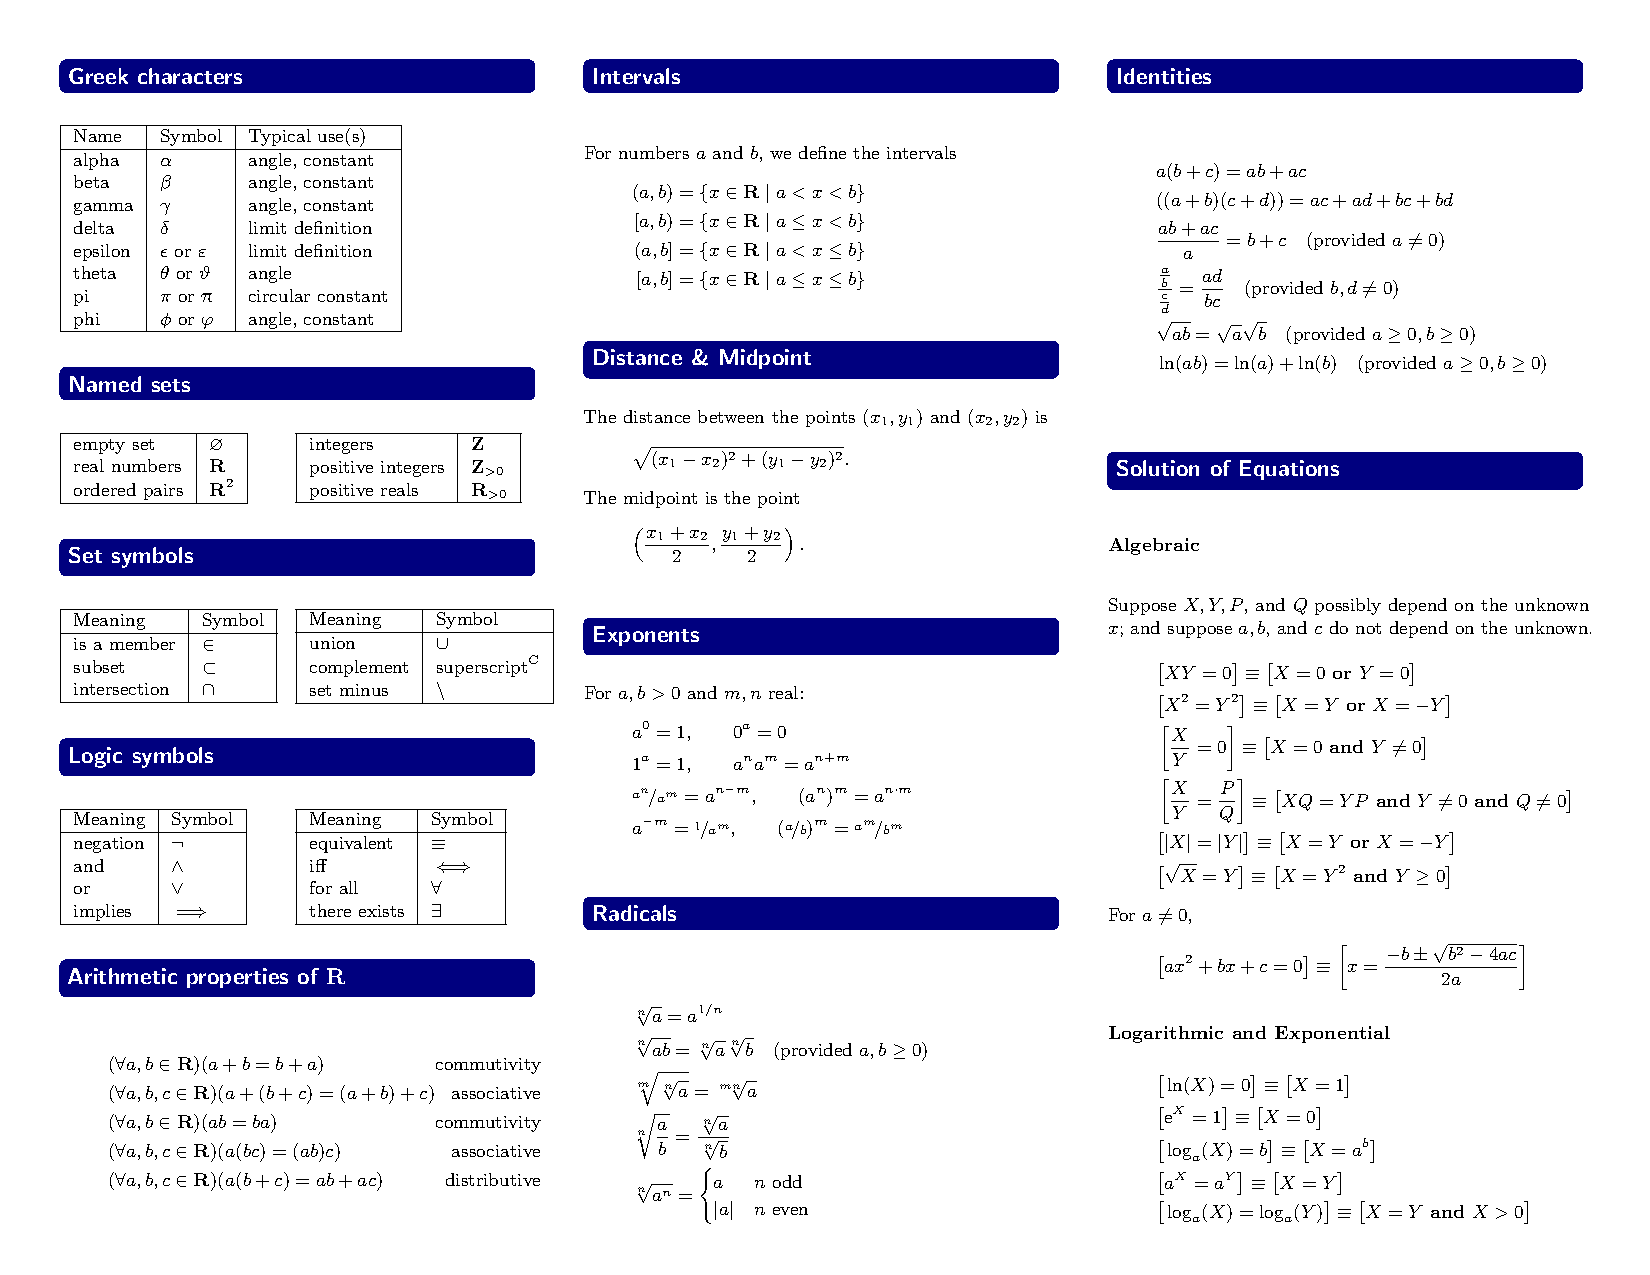
\includepdf[pages=-]{college-algebra-quick-reference.pdf}
\end{document}
